% GNUPLOT: LaTeX picture with Postscript
\documentclass{minimal}
% Set font size
\makeatletter
\def\@ptsize{1}
\InputIfFileExists{size11.clo}{}{%
   \GenericError{(gnuplot) \space\space\space\@spaces}{%
      Gnuplot Error: File `size11.clo' not found! Could not set font size%
   }{See the gnuplot documentation for explanation.%
   }{For using a font size a file `size<fontsize>.clo' has to exist.
        Falling back ^^Jto default fontsize 10pt.}%
  \def\@ptsize{0}
  \input{size10.clo}%
}%
\makeatother
% Load packages
\usepackage{calc}
\usepackage{graphicx}
\usepackage{color}
\usepackage[utf8x]{inputenc}
\makeatletter
% Select an appropriate default driver (from TeXLive graphics.cfg)
\begingroup
  \chardef\x=0 %
  % check pdfTeX
  \@ifundefined{pdfoutput}{}{%
    \ifcase\pdfoutput
    \else
      \chardef\x=1 %
    \fi
  }%
  % check VTeX
  \@ifundefined{OpMode}{}{%
    \chardef\x=2 %
  }%
\expandafter\endgroup
\ifcase\x
  % default case
  \PassOptionsToPackage{dvips}{geometry}
\or
  % pdfTeX is running in pdf mode
  \PassOptionsToPackage{pdftex}{geometry}
\else
  % VTeX is running
  \PassOptionsToPackage{vtex}{geometry}
\fi
\makeatother
% Set papersize
\usepackage[papersize={708.60bp,425.10bp},text={708.60bp,425.10bp}]{geometry}
% No page numbers and no paragraph indentation
\pagestyle{empty}
\setlength{\parindent}{0bp}%
% Load configuration file
\InputIfFileExists{gnuplot.cfg}{%
  \typeout{Using configuration file gnuplot.cfg}%
}{%
 \typeout{No configuration file gnuplot.cfg found.}%
}%
%
\begin{document}
\begingroup
  \makeatletter
  \providecommand\color[2][]{%
    \GenericError{(gnuplot) \space\space\space\@spaces}{%
      Package color not loaded in conjunction with
      terminal option `colourtext'%
    }{See the gnuplot documentation for explanation.%
    }{Either use 'blacktext' in gnuplot or load the package
      color.sty in LaTeX.}%
    \renewcommand\color[2][]{}%
  }%
  \providecommand\includegraphics[2][]{%
    \GenericError{(gnuplot) \space\space\space\@spaces}{%
      Package graphicx or graphics not loaded%
    }{See the gnuplot documentation for explanation.%
    }{The gnuplot epslatex terminal needs graphicx.sty or graphics.sty.}%
    \renewcommand\includegraphics[2][]{}%
  }%
  \providecommand\rotatebox[2]{#2}%
  \@ifundefined{ifGPcolor}{%
    \newif\ifGPcolor
    \GPcolorfalse
  }{}%
  \@ifundefined{ifGPblacktext}{%
    \newif\ifGPblacktext
    \GPblacktexttrue
  }{}%
  % define a \g@addto@macro without @ in the name:
  \let\gplgaddtomacro\g@addto@macro
  % define empty templates for all commands taking text:
  \gdef\gplbacktext{}%
  \gdef\gplfronttext{}%
  \makeatother
  \ifGPblacktext
    % no textcolor at all
    \def\colorrgb#1{}%
    \def\colorgray#1{}%
  \else
    % gray or color?
    \ifGPcolor
      \def\colorrgb#1{\color[rgb]{#1}}%
      \def\colorgray#1{\color[gray]{#1}}%
      \expandafter\def\csname LTw\endcsname{\color{white}}%
      \expandafter\def\csname LTb\endcsname{\color{black}}%
      \expandafter\def\csname LTa\endcsname{\color{black}}%
      \expandafter\def\csname LT0\endcsname{\color[rgb]{1,0,0}}%
      \expandafter\def\csname LT1\endcsname{\color[rgb]{0,1,0}}%
      \expandafter\def\csname LT2\endcsname{\color[rgb]{0,0,1}}%
      \expandafter\def\csname LT3\endcsname{\color[rgb]{1,0,1}}%
      \expandafter\def\csname LT4\endcsname{\color[rgb]{0,1,1}}%
      \expandafter\def\csname LT5\endcsname{\color[rgb]{1,1,0}}%
      \expandafter\def\csname LT6\endcsname{\color[rgb]{0,0,0}}%
      \expandafter\def\csname LT7\endcsname{\color[rgb]{1,0.3,0}}%
      \expandafter\def\csname LT8\endcsname{\color[rgb]{0.5,0.5,0.5}}%
    \else
      % gray
      \def\colorrgb#1{\color{black}}%
      \def\colorgray#1{\color[gray]{#1}}%
      \expandafter\def\csname LTw\endcsname{\color{white}}%
      \expandafter\def\csname LTb\endcsname{\color{black}}%
      \expandafter\def\csname LTa\endcsname{\color{black}}%
      \expandafter\def\csname LT0\endcsname{\color{black}}%
      \expandafter\def\csname LT1\endcsname{\color{black}}%
      \expandafter\def\csname LT2\endcsname{\color{black}}%
      \expandafter\def\csname LT3\endcsname{\color{black}}%
      \expandafter\def\csname LT4\endcsname{\color{black}}%
      \expandafter\def\csname LT5\endcsname{\color{black}}%
      \expandafter\def\csname LT6\endcsname{\color{black}}%
      \expandafter\def\csname LT7\endcsname{\color{black}}%
      \expandafter\def\csname LT8\endcsname{\color{black}}%
    \fi
  \fi
    \setlength{\unitlength}{0.0500bp}%
    \ifx\gptboxheight\undefined%
      \newlength{\gptboxheight}%
      \newlength{\gptboxwidth}%
      \newsavebox{\gptboxtext}%
    \fi%
    \setlength{\fboxrule}{0.5pt}%
    \setlength{\fboxsep}{1pt}%
    \definecolor{tbcol}{rgb}{1,1,1}%
\begin{picture}(14172.00,8502.00)%
      \csname LTb\endcsname%%
      \put(7086,8282){\makebox(0,0){\strut{}Tempo para realizar a}}%
      \put(7086,8102){\makebox(0,0){\strut{}Transformada de Fourier em função do tempo.}}%
    \gplgaddtomacro\gplbacktext{%
      \csname LTb\endcsname%%
      \put(1210,704){\makebox(0,0)[r]{\strut{}$0$}}%
      \put(1210,1360){\makebox(0,0)[r]{\strut{}$0.0005$}}%
      \put(1210,2016){\makebox(0,0)[r]{\strut{}$0.001$}}%
      \put(1210,2672){\makebox(0,0)[r]{\strut{}$0.0015$}}%
      \put(1210,3328){\makebox(0,0)[r]{\strut{}$0.002$}}%
      \put(1210,3984){\makebox(0,0)[r]{\strut{}$0.0025$}}%
      \put(1210,4641){\makebox(0,0)[r]{\strut{}$0.003$}}%
      \put(1210,5297){\makebox(0,0)[r]{\strut{}$0.0035$}}%
      \put(1210,5953){\makebox(0,0)[r]{\strut{}$0.004$}}%
      \put(1210,6609){\makebox(0,0)[r]{\strut{}$0.0045$}}%
      \put(1210,7265){\makebox(0,0)[r]{\strut{}$0.005$}}%
      \put(1210,7921){\makebox(0,0)[r]{\strut{}$0.0055$}}%
      \put(1342,484){\makebox(0,0){\strut{}$50$}}%
      \put(2106,484){\makebox(0,0){\strut{}$100$}}%
      \put(2870,484){\makebox(0,0){\strut{}$150$}}%
      \put(3634,484){\makebox(0,0){\strut{}$200$}}%
      \put(4397,484){\makebox(0,0){\strut{}$250$}}%
      \put(5161,484){\makebox(0,0){\strut{}$300$}}%
      \put(5925,484){\makebox(0,0){\strut{}$350$}}%
      \put(6689,484){\makebox(0,0){\strut{}$400$}}%
    }%
    \gplgaddtomacro\gplfronttext{%
      \csname LTb\endcsname%%
      \put(209,4312){\rotatebox{-270}{\makebox(0,0){\strut{}Tempo médio}}}%
      \put(4015,154){\makebox(0,0){\strut{}Número de pontos analisados}}%
      \csname LTb\endcsname%%
      \put(5702,7748){\makebox(0,0)[r]{\strut{}$\overline{t}(N)$}}%
    }%
    \gplgaddtomacro\gplbacktext{%
      \csname LTb\endcsname%%
      \put(8032,704){\makebox(0,0)[r]{\strut{}$0.01$}}%
      \put(8032,1735){\makebox(0,0)[r]{\strut{}$0.02$}}%
      \put(8032,2766){\makebox(0,0)[r]{\strut{}$0.03$}}%
      \put(8032,3797){\makebox(0,0)[r]{\strut{}$0.04$}}%
      \put(8032,4828){\makebox(0,0)[r]{\strut{}$0.05$}}%
      \put(8032,5859){\makebox(0,0)[r]{\strut{}$0.06$}}%
      \put(8032,6890){\makebox(0,0)[r]{\strut{}$0.07$}}%
      \put(8032,7921){\makebox(0,0)[r]{\strut{}$0.08$}}%
      \put(8164,484){\makebox(0,0){\strut{}$50$}}%
      \put(8966,484){\makebox(0,0){\strut{}$100$}}%
      \put(9767,484){\makebox(0,0){\strut{}$150$}}%
      \put(10569,484){\makebox(0,0){\strut{}$200$}}%
      \put(11370,484){\makebox(0,0){\strut{}$250$}}%
      \put(12172,484){\makebox(0,0){\strut{}$300$}}%
      \put(12973,484){\makebox(0,0){\strut{}$350$}}%
      \put(13775,484){\makebox(0,0){\strut{}$400$}}%
    }%
    \gplgaddtomacro\gplfronttext{%
      \csname LTb\endcsname%%
      \put(7295,4312){\rotatebox{-270}{\makebox(0,0){\strut{}Tempo médio}}}%
      \put(10969,154){\makebox(0,0){\strut{}Número de pontos analisados}}%
      \csname LTb\endcsname%%
      \put(12788,7748){\makebox(0,0)[r]{\strut{}$\sqrt(\overline{t})(N)$}}%
    }%
    \gplbacktext
    \put(0,0){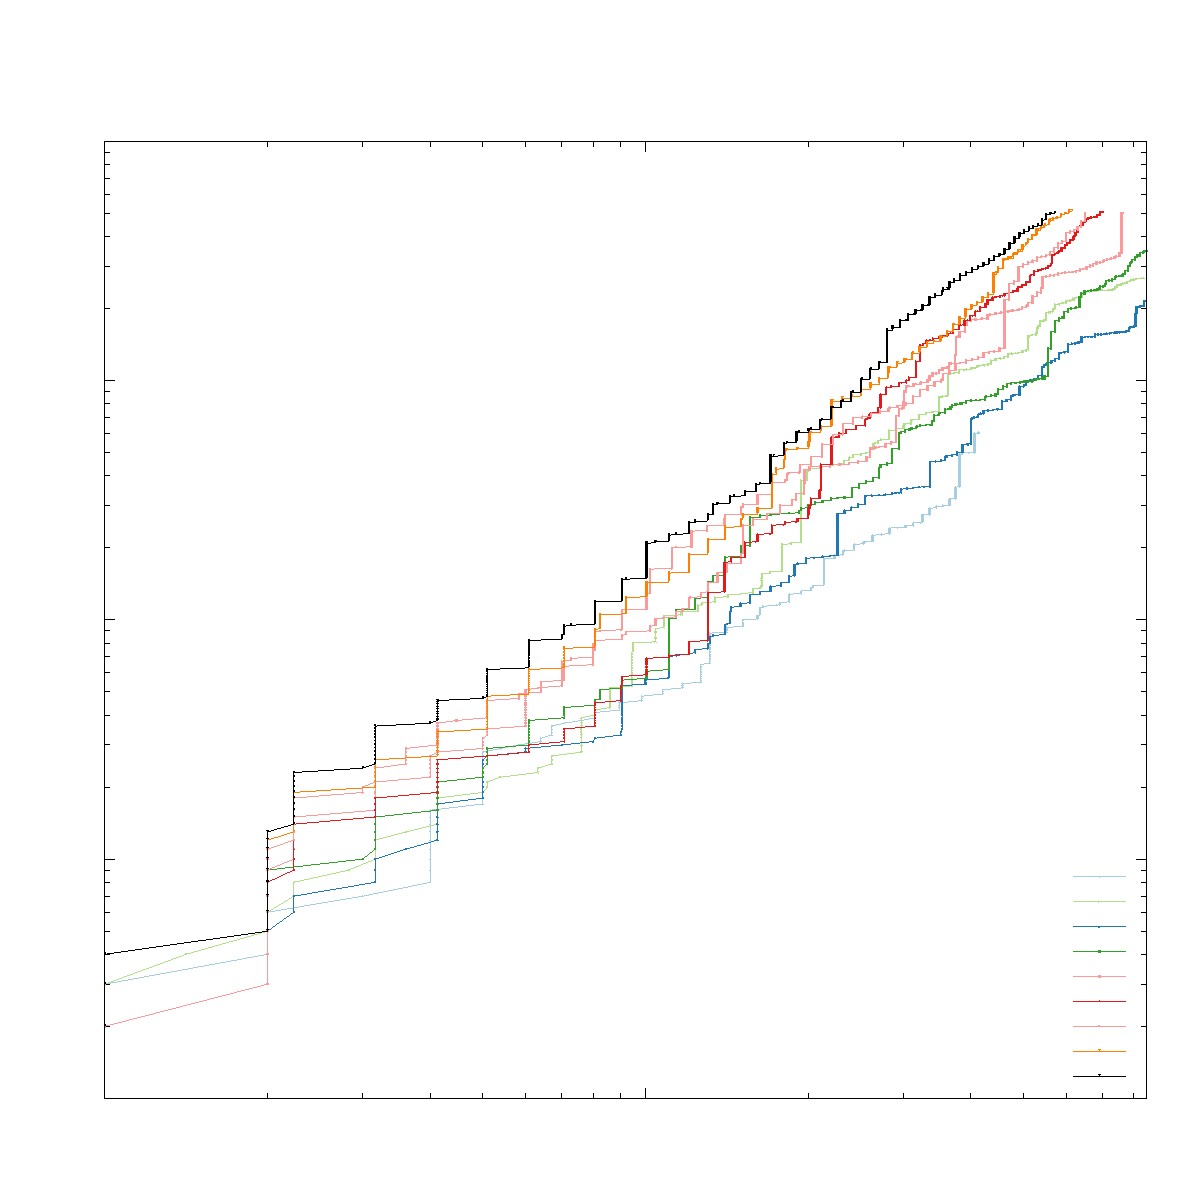
\includegraphics[width={708.60bp},height={425.10bp}]{tarefa-5-graf-11820833-inc}}%
    \gplfronttext
  \end{picture}%
\endgroup
\end{document}
